% ARPEGOS:  Automatized Roleplaying-game Profile Extensible Generator Ontology based System %
% Author : Alejandro Muñoz Del Álamo %
% Copyright 2019 %

% Section 4.3: Modelo de Comportamiento %
\section{Modelo de Comportamiento}
Después de describir los diferentes casos de uso de los requisitos del sistema, el próximo paso consiste
en elaborar el \textit{Modelo de Comportamiento}. Este modelo está comprendido por diagramas de secuencia 
del sistema, identificando operaciones y servicios del mismo. \medskip

Como varios diagramas de los mostrados en el apartado anterior tienen comportamientos 
muy parecidos, no se mostrarán todos los diagramas de secuencia, sino un conjunto reducido de éstos.\medskip

Otro detalle que cabe destacar es que no se puede concretar de qué manera interactúa el usuario con la aplicación 
en las vistas que dependen de la información del juego. Por tanto se hará uso de la función \textit{Interactuar()} 
para representar la interacción del usuario con el sistema en estos casos. Una vez finalizada 
la función, se considerará que el usuario ha realizado todas las acciones que haya estimado oportunas.

\subsection{Pantalla de selección}
Para mostrar una lista de selección, el sistema busca todos los elementos de la lista y 
la muestra. Una vez el usuario dispone de la lista de selección, el usuario puede 
elegir una opción (o varias, en función del elemento que se seleccione), quedando ésta 
marcada en la pantalla de selección.

\begin{figure}[H]
    \centering
    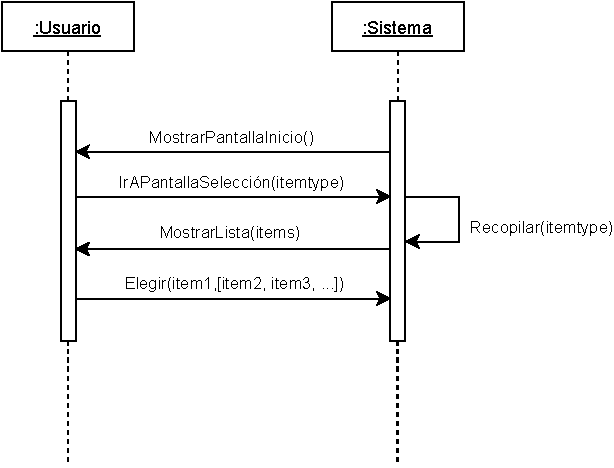
\includegraphics[scale=0.6]{Documentation-Scheme/Desarrollo/Análisis-Sistema/Comportamiento_Seleccion.pdf}
    \caption{Modelo de Comportamiento:Pantalla de selección}
    \label{Comportamiento_seleccion}
\end{figure}


\subsection{Crear personaje}
El proceso de creación de personajes puede considerarse el más complejo, pues debe ser dinámico para 
adaptarse a cualquiera de los juegos introducidos en la aplicación.\medskip

\begin{figure}[H]
    \centering
    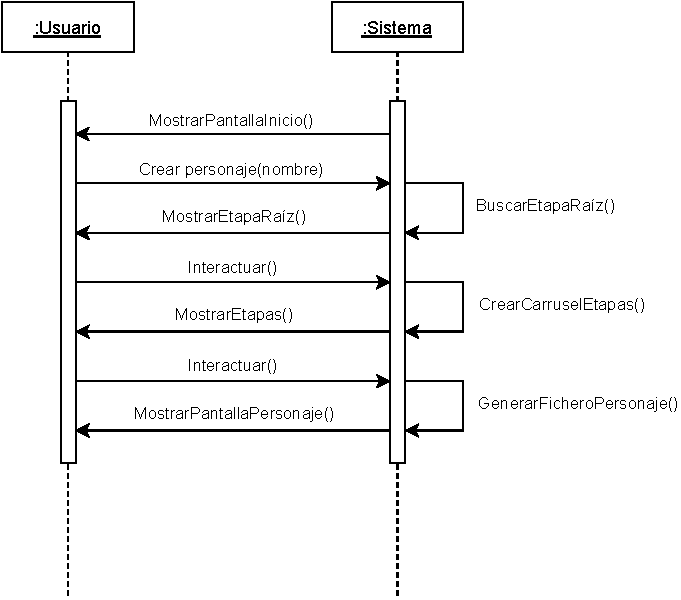
\includegraphics[scale=0.6]{Documentation-Scheme/Desarrollo/Análisis-Sistema/Comportamiento_Creacion.pdf}
    \caption{Modelo de Comportamiento: Crear personaje}
    \label{Comportamiento_creacion_personaje}
\end{figure}

\subsection{Editar personaje}
Para editar un personaje, será necesario haber accedido a la visualización del mismo, para que 
el usuario sea consciente de qué personaje es el que está editando.

\begin{figure}[H]
    \centering
    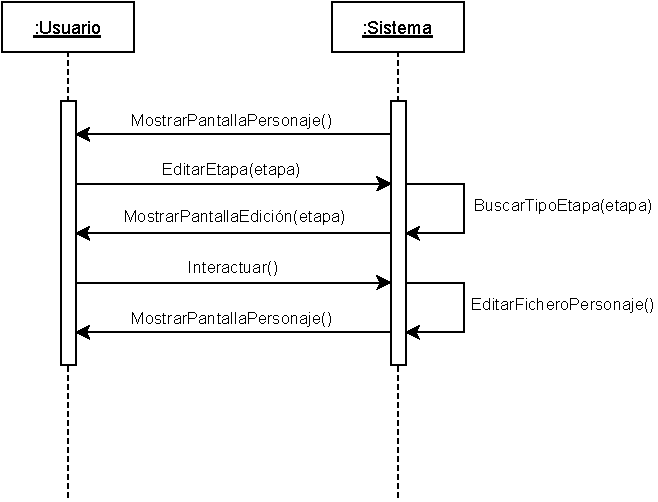
\includegraphics[scale=0.6]{Documentation-Scheme/Desarrollo/Análisis-Sistema/Comportamiento_Edicion.pdf}
    \caption{Modelo de Comportamiento: Editar personaje}
    \label{Comportamiento_edicion_personaje}
\end{figure}

\subsection{Eliminar personaje}
Al igual que en el caso anterior, será necesario haber accedido a la visualización del personaje antes de 
eliminarlo, de manera que el usuario sea consciente de qué personaje es el que está eliminando, ya que 
una vez hecho, no se podrá recuperar el fichero.

\begin{figure}[H]
    \centering
    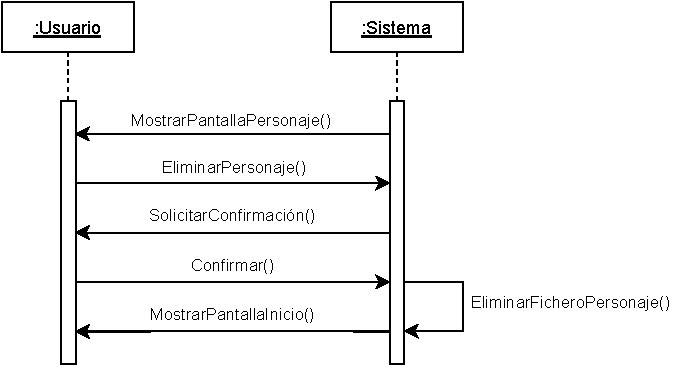
\includegraphics[scale=0.6]{Documentation-Scheme/Desarrollo/Análisis-Sistema/Comportamiento_Eliminacion.pdf}
    \caption{Modelo de Comportamiento: Eliminar personaje}
    \label{Comportamiento_eliminacion_personaje}
\end{figure}

\subsection{Cálculo de habilidades}
Para realizar el cálculo de habilidades, el usuario tendrá que indicar la habilidad que desea calcular 
y qué personaje la realiza para aplicar los valores correctos.

\begin{figure}[H]
    \centering
    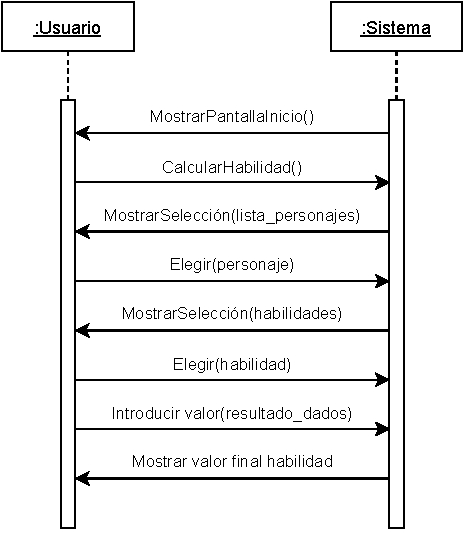
\includegraphics[scale=0.6]{Documentation-Scheme/Desarrollo/Análisis-Sistema/Comportamiento_Habilidades.pdf}
    \caption{Modelo de Comportamiento: Cálculo de habilidades}
    \label{Comportamiento_habilidades}
\end{figure}